\section{MMTP Algorithm}
\label{sec:alg}

The MMTP algorithm  is described in detail in Refs.~\cite{brian,steve}. The trigger algorithm is summarized here,
mostly to describe the adjustments made to utilize the algorithm with a cosmic muon detector.

The MMTP algorithm receives ADDC data and converts the ART addresses into Cartesian coordinates, look for subsets (``triggers'') which
 satisfy spatial and time prerequisites, and calculate quantities which characterize these triggers.
 The first step is referred to as the \textit{decoder}, the second step is referred to as the \textit{finder},
 and the third step is referred to as the \textit{fitter}.
 The present MMTP is firmware is synthesized and run on a Xilinx Virtex-7 FPGA in a VC707 evaluation board.
 

\subsection{Decoding}
\label{sec:alg-decode}

 The MMTP converts the VMM and strip numbers into Cartesian coordinates, rotated with respect to each other
  by the stereo angle
 for $X$, $U$, and $V$ planes, and 
 taking into consideration that some of the MM chambers are flipped relative to each other.
 
 The MMTP measures coordinates in units of strip pitch (400 $\mu$m).
 For example, if   strip 30 in VMM 5 is  converted into  a position 
 $x=$ 350 = $5*64 + 30$. 
 For each board, the algorithm uses the $z$-locations  listed in Table~\ref{tab:tab_1}.

\subsection{Finder}
\label{sec:alg-finder}
The next step of the MMTP algorithm is to search the data of all boards (at different $z$ positions)
for hits in given time window  and $x$ road.
The finder assigns hits in each board to a number of  $x$-roads, and evaluates
simultaneously if any road contains enough hits to generate a trigger.
Because our telescope accepts track with angle of incidence between -10$\deg$ and 25$\deg$, the algorithm uses
$x$-roads 1 VMM wide (1 VMM corresponds to 64 strips and 25.4 mm).

A road must contain at least two hits on the $X$ planes and at least two hits on the stereo ($UV$) planes to generate a trigger.
 Additionally, at least two of the hits on $X$ planes must occur on different quadruplets, to ensure a good slope resolution when
 later  fitting the $X$ hits with a straight line.

 Taking advantage of the low rate of ART signals, we use requirements looser than those ($3X$ and $3UV$)  anticipated in the
  NSW TDR to compensate for the MMFE8 board inefficiencies caused by the increasing number of VMM channels zapped by the
 Micromegas high voltage~\cite{noiseless}.
 A graphic visualisation of the finder algorithm is shown in Fig.~\ref{fig:cartoon_road_demo}.
%%%%%%%%%%%%%%%%%%%%%%%%%%%%%%%%%%%
\begin{figure}[!htpb]
  \begin{center}
    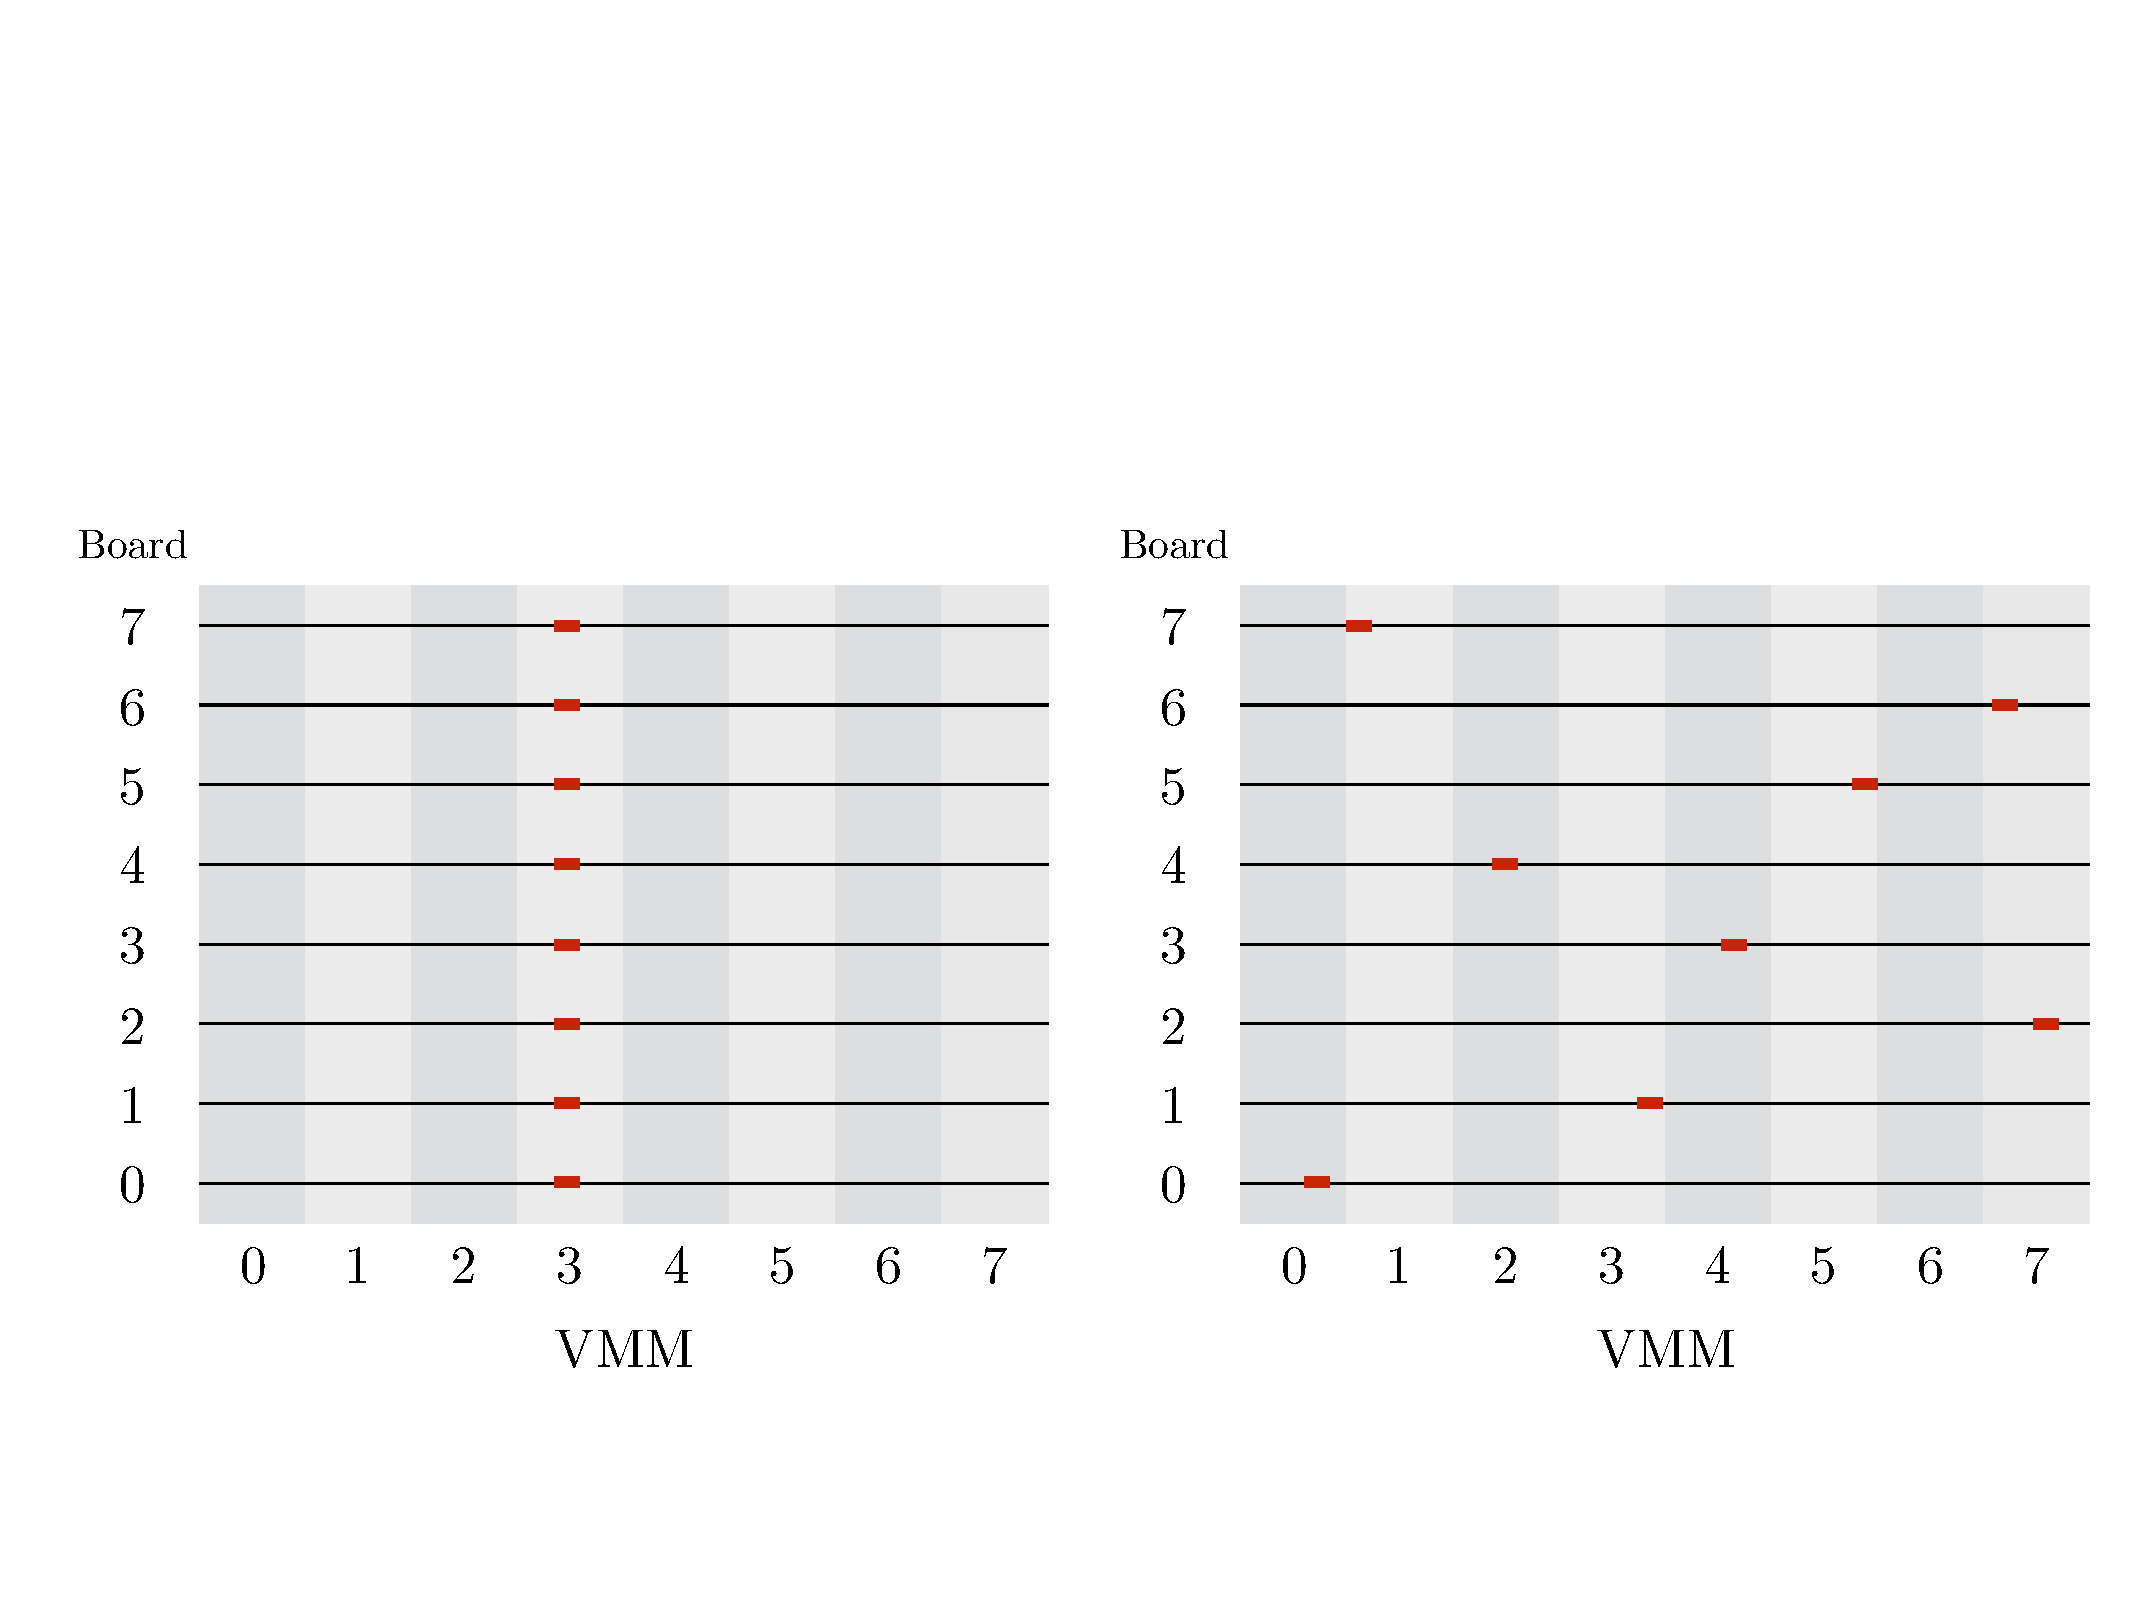
\includegraphics[width=1.0\textwidth]{figures/cartoons/cartoon_road_demo}
  \end{center}
  \vspace{-20pt}
  \caption{Hits generated by a cosmic muon passing through the octuplet (left) and
  randomly generated (right) as seen by the finder algorithm. Roads are 1-VMM wide and shown in alternating gray colors.
 Only the event on the left will generate a trigger.}
  \label{fig:cartoon_road_demo}
\end{figure}
%%%%%%%%%%%%%%%%%%%%%%%%%%%%%%%%%%%%%%%%%%%%%%
To recover those  cases in which a muon with a large angle of incidence deposits hits in two different roads, 
 the finder algorithm  also searches for  hits  in the 2 neighboring roads. 
 For example, road 3 uses hits from VMM 2, VMM 3, and VMM 4, so that the effective road size is 3 VMMs.


The finder also requires candidate hits to lie within a given time window in units of the BC clock.
Based on previous measurements of the time jitter of ART signal~\cite{oldart}, we  choose a 8 BC window~\footnote{Due to a timing bug in 
the MMTP firmware, this window  in Run 3522 is usually 7 and seldom 8 BCs. The bug was corrected prior to Runs 3527-3530. Runs are discussed 
in more detail in Section~\ref{sec:data-taking}.}.
 The time window is implemented as follows. A board hit in a given road is stored  for 8 BCs.
 No new hits are allowed in that road for that board until the hit is ``old'', i.e., after eight BCs.
 As new hits are entering into other boards in the same road, the trigger requirements are evaluated at every BC.
 Triggers are searched for in all roads simultaneously. 
 If a trigger is found in a road,
 a trigger is issued when the earliest hit in the road becomes ``old''. That trigger will carry the BCID of the ``old'' hit.

Each road can provide  one trigger per cycle of the BC clock. The triggers
 found  in all roads with the same BCID are placed in a road-number-based priority encoder  and sent sequentially to the fitter for further calculations.
 Because the MMTP clock is eight times faster than the BC clock, the fitter can process close to 8 triggers.
 In our case,  no found trigger is lost.
\subsection{Fitter}
\label{sec:alg-fitter}
The  \textit{fitter} algorithm  provides the location and quality of a trigger.
The location is represented by a point in the  $\eta-\phi$ space which in the NSW upgrade is used by downstream
trigger modules to define the L1 muon trigger region of interest (ROI).

In ATLAS, the global slopes are calculated as  $m_l = \, <x_l/z_l> $. For each hit
  in $l=X$ or $l=U$ or $l=V$ planes, the quantity $x_l/z_l$ , where $x_l$ is the coordinate value
 and $z_l$ is the  distance  from the interaction point ($\simeq$750 cm), is returned by look-up-tables (LUT).
 Averages are calculated by the fitter algorithm.
The 3 slopes are converted with look up tables which 
 return  $m_y=\frac{m_U - m_V}{2\ \text{tan}(\theta_\text{stereo})}$ and $\eta$, $\phi$ coordinates from the $m_x,m_y$ values.

 In parallel,  the algorithm also fits  all hits in the $X$-planes with a straight line 
 returning a local slope $m_x^l$. A cut on the slope difference  $\Delta\theta = |\theta_g - \theta_l |$, the angles derived from
 the $m_x$ and $m_x^l$ slopes,  is supposed to be used to reduce the rate of accidental triggers 


Since cosmic muons do not originate from a point-like source, the fitter algorithm has been modified to use strip numbers instead of slopes
(we use a new LUT which does not divide $x$ by the distance from the interaction point).
The local slope is evaluated as    $m_x^\text{local} = \sum c_i \ x_i$, where the sum includes all $X$ hits, and $c_i$ are constants,
stored in a new LUT, which depend on the $z$ position of the $X$ plane (see Table~1) in units of strip pitch. 
 The detector distance from the beamline is set to 0.
 Instead of the global slope, the algorithm evaluates $<x_l>$ and $<z_l>$ for $l=X,U,V$ hits separately.

 Once a trigger has been processed, our algorithm stores: a) the ADDC data in 15 BC preceding the trigger BCID; b) the trigger BCID, the address of the hits
 providing a trigger, the local slope, and other ancillary information; and c) the BCID of a scintillator trigger into 3 different FIFO,
 the content of which is transmitted as UDP packets
 in round-robin mode and recorded.
 
\subsection{Method for evaluating the MMTP performance}
\label{sec:alg-resol}

 We check the MMTP performance by using events in which we can reconstruct a track using Micromegas clusters.
 The cluster selection is described in Ref.~\cite{noisy}. In particular, the  BCID of the hits forming a cluster is required
 to be in a 15 BC window around the BCID of the scintillator trigger.
 As explained in Ref.~\cite{noisy}, we fit the available cluster with two straight lines in the $x-z$ and $y-z$ planes.
 The fits, referred to as MM fits, are performed in the same coordinate system as the MMTP. The fits provide slopes, $M_X$ and $M_Y$, and intercepts, $A_X$ and $A_Y$,
 which are used to set limits to the MMTP space resolution. In the fair assumption that the uncertainty of the parameters returned by the MM fits 
  are negligible,  comparisons with MMTP results measure its accuracy.

  We select tracks the clusters of which satisfy the trigger requirements. The number of MMTP triggers found in the latter
 set measures the MMTP efficiency.

 To measure the angular resolution  we compare the MMTP $<x_X>$  to  $A_X$+ $M_X <z_X>$.
  The rms value of this difference, referred to as  $x_{\rm TP}-x_{\rm MM}$,
  when divided by 750 cm, yields the $m_x$ resolution.

 We also evaluate the MMTP accuracy in measuring the $y$ coordinate. We extrapolate the MMTP $<x_U>$,$< x_V>$, $<x_V>$ values to
 a common $z_c$ value using the slope value returned by the MM fit. At that $z_c$, we evaluate $y_{\rm TP}$
 as   $\frac{x_U - x_V}{2\ \text{tan}(\theta_\text{stereo})}$ or  $\frac{x_X - x_V(U)}{\ \text{tan}(\theta_\text{stereo})}$
 or  $\frac{x_X - x_V(V)}{\ \text{tan}(\theta_\text{stereo})}$ (we average the various values).
 We then  compare  $y_{\rm TP}$ to  $y_{\rm MM}$ derived from the MM fit at the same $z$. The rms value of distribution
 of their difference divided by the detector strip length is suggestive of the achievable $\phi$ segmentation.  

 The distribution of the difference between angles corresponding to the slope of the MMTP local fit and that corresponding to $M_x$,
 referred to as $\theta_{\rm local}-\theta_{\rm MM} $,
 provides a measure of the resolution of the MMTP local fit.
  


